\documentclass{beamer}

\usepackage[utf8]{inputenc}
\usepackage{tabularx}
\usepackage{amsmath}
\usepackage{amssymb}
\usepackage{booktabs}
\usepackage{hyperref}
\usepackage{graphicx}
\usepackage{multicol}
\graphicspath{{pics/}}

\usetheme{Warsaw}
\usefont{professionalfonts}

\title{Equivalent metrics}

\author{Anthony Catterwell}

\institute{University of Edinburgh}

\begin{document}

\begin{frame}
    \maketitle
\end{frame}

\begin{frame}{Overview}
    \tableofcontents
\end{frame}

\section{Metric spaces}

\subsection{What constitutes a metric space?}

\begin{frame}{What constitutes a metric space?}
    \begin{definition}
        A set $X$ with function
        $d: X \times X \rightarrow \mathbb{R}$
        which $\forall x, y, z \in X$ satisfy
        \begin{align*}
            \text{\textsc{Positive Definite: }}   & d(x,y) \geq 0 \ \text{and} \\
                                                  & d(x,y) = 0 \iff x = y \\
            \text{\textsc{Symmetric: }}           & d(x,y) = d(y,x) \\
            \text{\textsc{Triangle Inequality: }} & d(x,y) \leq d(x,z) + d(z,y) \\
        \end{align*}
    \end{definition}
\end{frame}

\subsection{Some metrics of $R^2$}

\begin{frame}{Some metrics of $R^2$}
    \begin{block}{}
        \begin{align*}
            \text{Manhattan distance} \quad & d_1(\textbf{x},\textbf{y}) :=
            |x_1 - y_1| + |x_2 - y_2| \\
            \text{Euclidean distance} \quad & d_2(\textbf{x},\textbf{y}) :=
            \sqrt{(x_1 - y_1)^2 + (x_2 - y_2)^2} \\
            % \text{Discrete metric} \quad &d_3(x,y) := 
            % \begin{cases}{}
            % 	0 & x = y \\
            % 	1 & x \neq y\\
            % \end{cases}\\
        \end{align*}
        \end{block}
        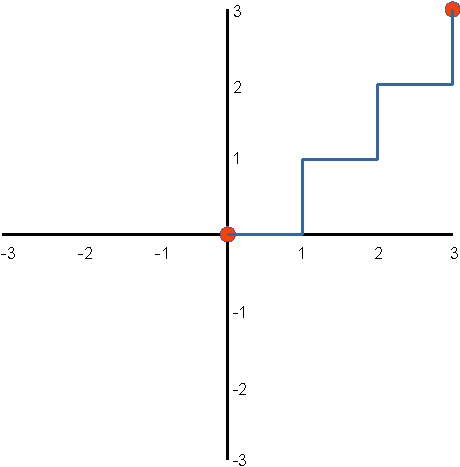
\includegraphics[height=80]{graph2.pdf} \quad
        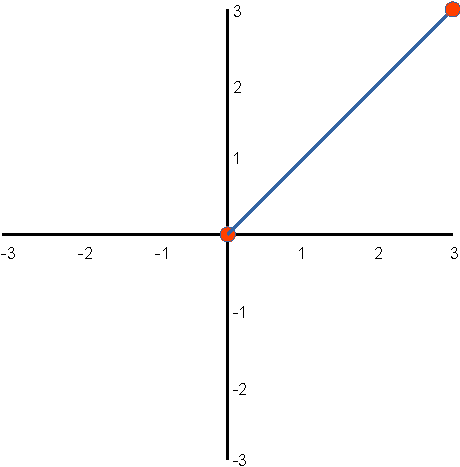
\includegraphics[height=80]{graph1.pdf}

    \end{frame}

    \subsection{Are they equivalent?}
    \begin{frame}{Are they equivalent?}

        \begin{block}
            $d_1(\textbf{x},\textbf{y}) := |x_1 - y_1| + |x_2 - y_2|$ \\

            $d_2(\textbf{x},\textbf{y}) := \sqrt{(x_1 - y_1)^2 + (x_2 - y_2)^2}$
            % $d_3(\textbf{x},\textbf{y}) := d_0(x_1,y_1) + d_0(x_2,y_2)$
        \end{block}

        \begin{tabular}{r|c c c c c}
        & $O:(0,0)$ & $(4,0)$ & $(15,18)$ & $(57,42)$ & $(900,600)$ \\
        \hline \\
            $d_1(O,x)$ & 0 & 4 & 23 & 99 & 1500 \\
            $d_2(O,x)$ & 0 & 4 & 33 & 71 & 1082 \\
            % $d_3(O,x)$ & 0 & 1 & 1  & 1  & 1    \\
        \end{tabular}

        \pause

        \begin{itemize}
            \item $d_1$ and $d_2$ seem to increase proportionally with each other.\\
            \item Characteristic of equivalent metrics.
        \end{itemize}

    \end{frame}

    \section{Equivalence}

    \subsection{Definition}

    \begin{frame}{Definition}
        There are several ways to express metric equivalence.
        \begin{definition}{}
            $d_1$ and $d_2$ in $X$ are said to be \emph{equivalent} if
            $\forall \epsilon > 0 \ \exists \delta > 0$ such that
            $$d_1(x,y) < \delta \implies d_2(x,y) < \epsilon$$
            $\forall x,y \in X$, and vice-versa.
        \end{definition}
        % which is to say:
        % two points that are close under one metric, are must also  be close in the other.
    \end{frame}

    \subsection{Other ways of expressing equivalence}
    \begin{frame}{Open balls}

        \begin{definition}{}
            An open ball $B_r(x;d)$ in a metric space $(X,d)$ is defined as
            $$\{y \in X : d(x,y) < r\}$$
        \end{definition}
        \pause
        \begin{theorem}{}
            The metrics $d_1$ and $d_2$ on a set $X$ are equivalent iff
            $$\forall \epsilon > 0 \ \exists \delta > 0 \ . \ B_\delta(x;d_1) \subseteq B_\epsilon(x;d_2)$$
            in their corresponding metric spaces $(X,d_1)$ and $(X,d_2)$.\\
            And vice-versa.
        \end{theorem}

    \end{frame}

    \begin{frame}{Balls (cont.)}
        Relating back to our example with Manhattan metric $d_1$ and Euclidean metric $d_2$ in $\mathbb{R}^2$:
        \begin{block}{}
            \centering
            \begin{tabular}{c c}
                $B_r(O,d_1)$ & $B_r(O,d_2)$ \\
                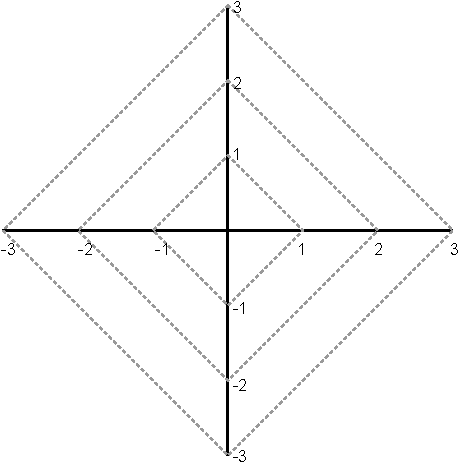
\includegraphics[height=120]{balls2.pdf} & 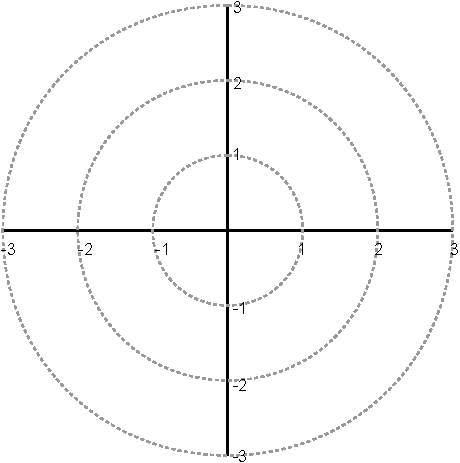
\includegraphics[height=120]{balls1.pdf}\\
            \end{tabular}
            \forall r \in \{0,1,2,3\}
        \end{block}
    \end{frame}

    \begin{frame}{Balls (cont. 2)}
        Overlaying them, you can see how $d_1$ and $d_2$ could be equivalent.\\
        \centering
        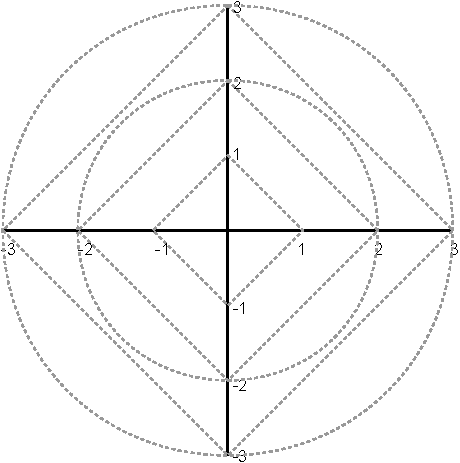
\includegraphics[height=180]{nest.pdf}\\
    \end{frame}

    \begin{frame}{Open sets}
        \begin{definition}{}
            A set $V \subseteq X$ is said to be \emph{open} if and only if
            $$\forall x \in V \ \exists \epsilon > 0 \ . \ B_\epsilon(x) \subseteq V$$
        \end{definition}
        \pause
        \begin{theorem}{}
            Metrics $d_1$ and $d_2$ on a set $X$ are equivalent if and only if
            $$A \subseteq X \text{ is open under } d_1 \iff A \text{ is open under } d_2.$$
        \end{theorem}

        % The proof of this follows from the interpretation of equivalence with balls.
    \end{frame}

    \subsection{Strong equivalence}
    \begin{frame}{Strong equivalence}
        Strong equivalence is a \emph{sufficient} condition for equivalence.
        \begin{definition}{}
            Two metrics $d_1$ and $d_2$ are said to be \emph{strongly equivalent} if
            $\exists \alpha, \beta \in \mathbb{R^+} \text{such that}$
            $$d_1(x,y) \le \alpha\cdot d_2(x,y) \quad \text{and} \quad d_2(x,y) \le \beta\cdot d_1(x,y)$$
        \end{definition}
    \item Somewhat analogous to continuity vs uniform continuity.
    \end{frame}

    \begin{frame}{Manhattan and Euclidean distance are strongly equivalent}
        $d_1(\textbf{x},\textbf{y}) &:= |x_1 - y_1| + |x_2 - y_2|$\\
        $d_2(\textbf{x},\textbf{y}) &:= \sqrt{(x_1 - y_1)^2 + (x_2 - y_2)^2}$\\

        \begin{proof}{}
            Let $a,b = x_1-y_1,\ x_2-y_2$. Then
            \begin{align*}{}
            &d_1(\textbf{x},\textbf{y})^2 = a^2 + b^2 \quad \text{and} \quad d_2(\textbf{x},\textbf{y})^2 = a^2 + b^2 + 2ab\\
                \implies &d_1(\textbf{x},\textbf{y}) \le 1\cdot d_2(\textbf{x},\textbf{y})
            \end{align*}
            Since we have $ab \le \max(a, b)^2$
            \begin{align*}{}
            &\implies 2ab \le 2(a^2 + b^2)\\
            &\implies a^2 + b^2 + 2ab \le 3(a^2 + b^2)\\
            &\implies d_2(\textbf{x},\textbf{y}) \le \sqrt{3}\cdot d_1(\textbf{x},\textbf{y})
            \end{align*}
        \end{proof}

    \end{frame}

    \section{Epilogue}
    \begin{frame}{Epilogue}
        Might be tempting to think that 
        \begin{block}{}
            If $d_1$ and $d_2$ are equivalent then $\forall a,b,c \in X$
            $$d_1(a,b) \le d_1(a,c) \implies d_2(a,b) \le d_2(a,c)$$
        \end{block}
        \pause
        \begin{alertblock}{}
            Holds for the majority of cases, but not generally true!
        \end{alertblock}
        \pause
        Take (2,2) and (3,0) with Manhattan and Euclidean distance metrics $d_1$ and $d_2$.\\
        $$d_1(O,(3,0)) = 3 < d_1(O,(2,2)) = 4$$
        \pause
        but
        $$d_2(O,(3,0)) = 3 \alert{>} d_2(O(2,2)) = 2.8$$
    \end{frame}

    \begin{frame}{}
        \centering
        \Huge{Thanks!}
    \end{frame}

    \end{document}
